\documentclass[10pt]{article}
\usepackage[T1]{fontenc}
\usepackage{lmodern}
\usepackage{mathtools}
\usepackage{booktabs}
\usepackage{adjustbox}
\usepackage[left=1.5cm, right=2cm, top=1.5cm, bottom=2cm]{geometry}
\usepackage{tikz}
\usepackage{pgfplots}
\pgfplotsset{compat=1.18}
\usetikzlibrary{arrows.meta,positioning,calc}
\setlength\parindent{0pt}
\title{g7 3 - No Protection - Benchmarking Algorithm - Ascending}
\date{}
\author{}

\begin{document}
\maketitle
\section*{Topology}
\begin{center}\begin{adjustbox}{max width=\linewidth}
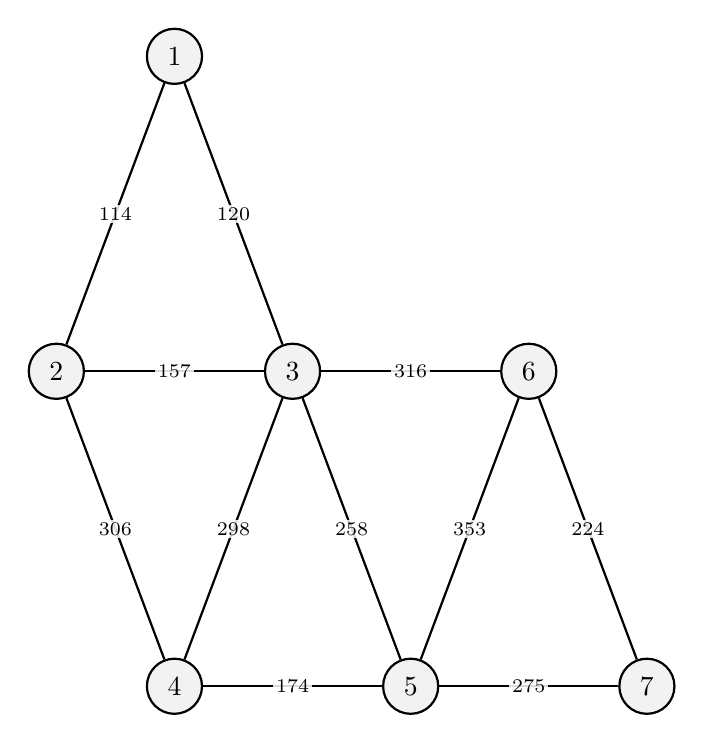
\begin{tikzpicture}[baseline, >={Stealth[length=2mm]},
  netnode/.style={circle, draw, thick, fill=gray!10, minimum size=7mm, inner sep=1pt},
  link/.style={thick},
  linklabel/.style={font=\scriptsize, inner sep=1pt, fill=white, fill opacity=0.85, text opacity=1}]
\node[netnode] (S1) at (1.500,8.000) {1};
\node[netnode] (S2) at (0.000,4.000) {2};
\node[netnode] (S3) at (3.000,4.000) {3};
\node[netnode] (S4) at (1.500,0.000) {4};
\node[netnode] (S5) at (4.500,0.000) {5};
\node[netnode] (S6) at (6.000,4.000) {6};
\node[netnode] (S7) at (7.500,0.000) {7};
\draw[link] (S1) to node[linklabel] {114} (S2);
\draw[link] (S1) to node[linklabel] {120} (S3);
\draw[link] (S2) to node[linklabel] {157} (S3);
\draw[link] (S2) to node[linklabel] {306} (S4);
\draw[link] (S3) to node[linklabel] {298} (S4);
\draw[link] (S3) to node[linklabel] {258} (S5);
\draw[link] (S3) to node[linklabel] {316} (S6);
\draw[link] (S4) to node[linklabel] {174} (S5);
\draw[link] (S5) to node[linklabel] {353} (S6);
\draw[link] (S5) to node[linklabel] {275} (S7);
\draw[link] (S6) to node[linklabel] {224} (S7);
\end{tikzpicture}
\end{adjustbox}\end{center}
\section*{Performance Parameters}
\begin{center}\begin{tabular}{lr}
\toprule
Highest link load & 467 Gb/s \\
Highest used FSU & 130 / 320 \\
Total used FSUs & 126 \\
Transponder cost & 66.0 \\
\midrule
SC-DP-QPSK transponders & 36 \\
SC-DP-16QAM transponders & 6 \\
DP-16QAM transponders & 0 \\
\bottomrule
\end{tabular}\end{center}
\clearpage
\section*{Link Load Map}
\begin{center}\begin{adjustbox}{max width=\linewidth}
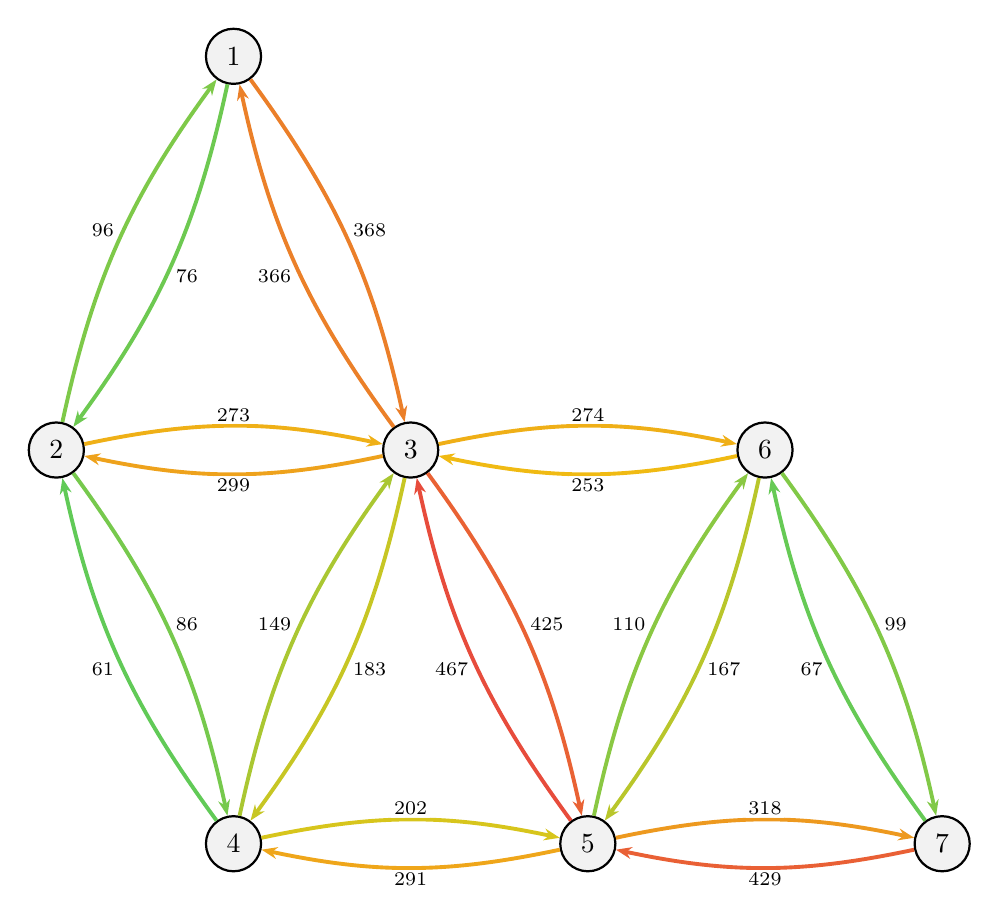
\begin{tikzpicture}[baseline, >={Stealth[length=2mm]},
  netnode/.style={circle, draw, thick, fill=gray!10, minimum size=7mm, inner sep=1pt},
  link/.style={line width=1.4pt},
  linklabel/.style={font=\scriptsize, inner sep=1pt, fill=white, fill opacity=0.85, text opacity=1}]
\node[netnode] (S1) at (2.250,10.000) {1};
\node[netnode] (S2) at (0.000,5.000) {2};
\node[netnode] (S3) at (4.500,5.000) {3};
\node[netnode] (S4) at (2.250,0.000) {4};
\node[netnode] (S5) at (6.750,0.000) {5};
\node[netnode] (S6) at (9.000,5.000) {6};
\node[netnode] (S7) at (11.250,0.000) {7};
\draw[link, ->, draw={rgb,255:red,109;green,201;blue,81}] (S1) to[bend left=12] node[linklabel, auto] {76} (S2);
\draw[link, ->, draw={rgb,255:red,235;green,127;blue,41}] (S1) to[bend left=12] node[linklabel, auto] {368} (S3);
\draw[link, ->, draw={rgb,255:red,126;green,201;blue,73}] (S2) to[bend left=12] node[linklabel, auto] {96} (S1);
\draw[link, ->, draw={rgb,255:red,239;green,176;blue,23}] (S2) to[bend left=12] node[linklabel, auto] {273} (S3);
\draw[link, ->, draw={rgb,255:red,118;green,201;blue,77}] (S2) to[bend left=12] node[linklabel, auto] {86} (S4);
\draw[link, ->, draw={rgb,255:red,235;green,128;blue,41}] (S3) to[bend left=12] node[linklabel, auto] {366} (S1);
\draw[link, ->, draw={rgb,255:red,238;green,162;blue,28}] (S3) to[bend left=12] node[linklabel, auto] {299} (S2);
\draw[link, ->, draw={rgb,255:red,199;green,198;blue,36}] (S3) to[bend left=12] node[linklabel, auto] {183} (S4);
\draw[link, ->, draw={rgb,255:red,233;green,98;blue,52}] (S3) to[bend left=12] node[linklabel, auto] {425} (S5);
\draw[link, ->, draw={rgb,255:red,239;green,175;blue,23}] (S3) to[bend left=12] node[linklabel, auto] {274} (S6);
\draw[link, ->, draw={rgb,255:red,97;green,202;blue,87}] (S4) to[bend left=12] node[linklabel, auto] {61} (S2);
\draw[link, ->, draw={rgb,255:red,170;green,199;blue,50}] (S4) to[bend left=12] node[linklabel, auto] {149} (S3);
\draw[link, ->, draw={rgb,255:red,215;green,197;blue,28}] (S4) to[bend left=12] node[linklabel, auto] {202} (S5);
\draw[link, ->, draw={rgb,255:red,231;green,76;blue,60}] (S5) to[bend left=12] node[linklabel, auto] {467} (S3);
\draw[link, ->, draw={rgb,255:red,239;green,166;blue,26}] (S5) to[bend left=12] node[linklabel, auto] {291} (S4);
\draw[link, ->, draw={rgb,255:red,138;green,200;blue,67}] (S5) to[bend left=12] node[linklabel, auto] {110} (S6);
\draw[link, ->, draw={rgb,255:red,237;green,153;blue,31}] (S5) to[bend left=12] node[linklabel, auto] {318} (S7);
\draw[link, ->, draw={rgb,255:red,240;green,186;blue,19}] (S6) to[bend left=12] node[linklabel, auto] {253} (S3);
\draw[link, ->, draw={rgb,255:red,185;green,198;blue,43}] (S6) to[bend left=12] node[linklabel, auto] {167} (S5);
\draw[link, ->, draw={rgb,255:red,129;green,201;blue,71}] (S6) to[bend left=12] node[linklabel, auto] {99} (S7);
\draw[link, ->, draw={rgb,255:red,233;green,96;blue,53}] (S7) to[bend left=12] node[linklabel, auto] {429} (S5);
\draw[link, ->, draw={rgb,255:red,102;green,202;blue,85}] (S7) to[bend left=12] node[linklabel, auto] {67} (S6);
\end{tikzpicture}
\end{adjustbox}\end{center}
\begin{center}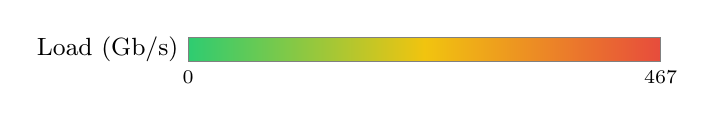
\begin{tikzpicture}
\definecolor{scalelow}{RGB}{46,204,113}\definecolor{scalemid}{RGB}{241,196,15}\definecolor{scalehigh}{RGB}{231,76,60}
\shade[left color=scalelow, right color=scalemid] (0,0) rectangle (3,0.3);
\shade[left color=scalemid, right color=scalehigh] (3,0) rectangle (6,0.3);
\draw[gray] (0,0) rectangle (6,0.3);
\node[below, font=\scriptsize] at (0,0) {0};
\node[below, font=\scriptsize] at (6,0) {467};
\node[left, font=\small] at (0,0.15) {Load (Gb/s)};
\end{tikzpicture}\end{center}
\section*{Link Load Distribution}

\begin{center}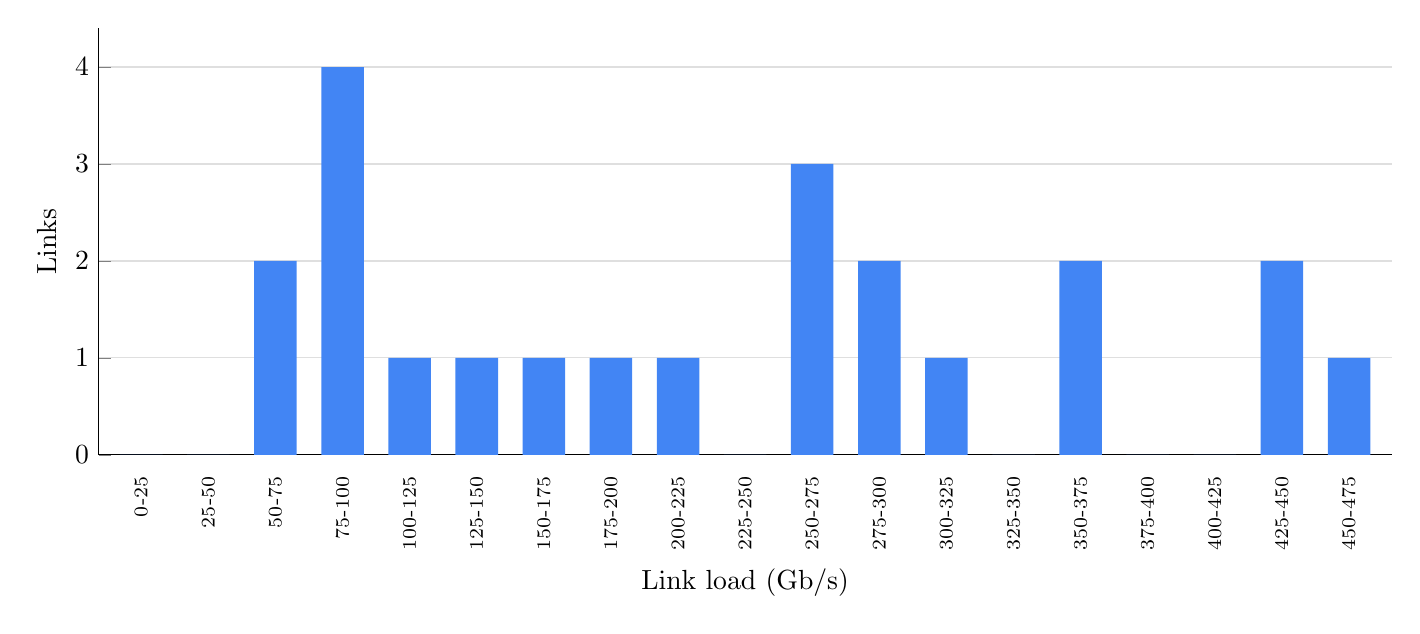
\begin{tikzpicture}
\begin{axis}[
  ybar, bar width=0.540cm, width=18.000cm, height=7cm,
  ymin=0, ymajorgrids, grid style={gray!25}, axis lines*=left,
  enlarge x limits={abs=0.540cm}, xtick=data, major x tick style={draw=none},
  x tick label style={rotate=90, font=\scriptsize, /pgf/number format/1000 sep=},
  legend style={at={(0.5,-0.3)}, anchor=north, legend columns=-1, draw=none},
  ylabel={Links},
  xlabel={Link load (Gb/s)},
  symbolic x coords={0-25,25-50,50-75,75-100,100-125,125-150,150-175,175-200,200-225,225-250,250-275,275-300,300-325,325-350,350-375,375-400,400-425,425-450,450-475}]
\addplot[fill={rgb,255:red,66;green,133;blue,244}, draw=none] coordinates {(0-25,0.000) (25-50,0.000) (50-75,2.000) (75-100,4.000) (100-125,1.000) (125-150,1.000) (150-175,1.000) (175-200,1.000) (200-225,1.000) (225-250,0.000) (250-275,3.000) (275-300,2.000) (300-325,1.000) (325-350,0.000) (350-375,2.000) (375-400,0.000) (400-425,0.000) (425-450,2.000) (450-475,1.000) };
\end{axis}
\end{tikzpicture}\end{center}
\clearpage
\section*{Spectrum Occupancy}
\begin{center}\begin{adjustbox}{max width=\linewidth}
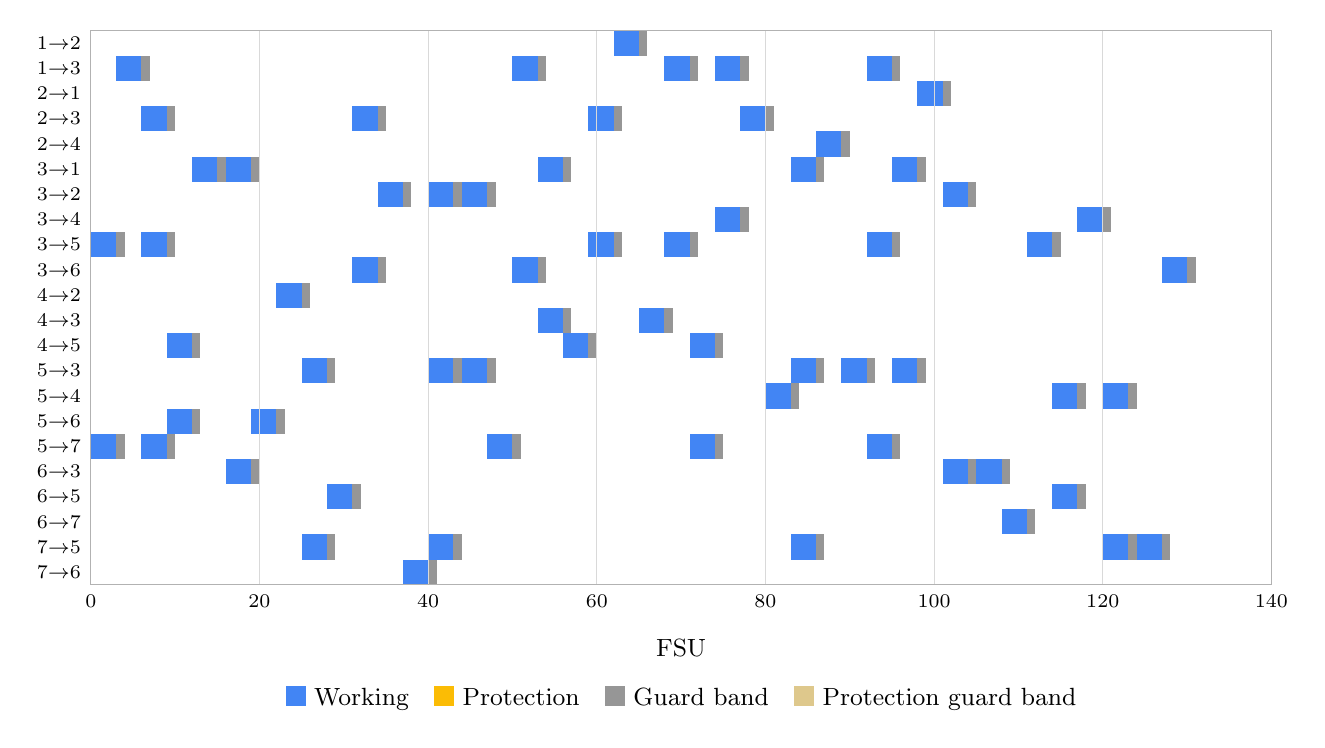
\begin{tikzpicture}[x=0.1071cm, y=-0.32cm]
\fill[fill={rgb,255:red,66;green,133;blue,244}] (62,0) rectangle (65,1);
\fill[fill={rgb,255:red,150;green,150;blue,150}] (65,0) rectangle (66,1);
\node[left, font=\scriptsize] at (0,0.5) {1\(\to\)2};
\fill[fill={rgb,255:red,66;green,133;blue,244}] (3,1) rectangle (6,2);
\fill[fill={rgb,255:red,150;green,150;blue,150}] (6,1) rectangle (7,2);
\fill[fill={rgb,255:red,66;green,133;blue,244}] (50,1) rectangle (53,2);
\fill[fill={rgb,255:red,150;green,150;blue,150}] (53,1) rectangle (54,2);
\fill[fill={rgb,255:red,66;green,133;blue,244}] (68,1) rectangle (71,2);
\fill[fill={rgb,255:red,150;green,150;blue,150}] (71,1) rectangle (72,2);
\fill[fill={rgb,255:red,66;green,133;blue,244}] (74,1) rectangle (77,2);
\fill[fill={rgb,255:red,150;green,150;blue,150}] (77,1) rectangle (78,2);
\fill[fill={rgb,255:red,66;green,133;blue,244}] (92,1) rectangle (95,2);
\fill[fill={rgb,255:red,150;green,150;blue,150}] (95,1) rectangle (96,2);
\node[left, font=\scriptsize] at (0,1.5) {1\(\to\)3};
\fill[fill={rgb,255:red,66;green,133;blue,244}] (98,2) rectangle (101,3);
\fill[fill={rgb,255:red,150;green,150;blue,150}] (101,2) rectangle (102,3);
\node[left, font=\scriptsize] at (0,2.5) {2\(\to\)1};
\fill[fill={rgb,255:red,66;green,133;blue,244}] (6,3) rectangle (9,4);
\fill[fill={rgb,255:red,150;green,150;blue,150}] (9,3) rectangle (10,4);
\fill[fill={rgb,255:red,66;green,133;blue,244}] (31,3) rectangle (34,4);
\fill[fill={rgb,255:red,150;green,150;blue,150}] (34,3) rectangle (35,4);
\fill[fill={rgb,255:red,66;green,133;blue,244}] (59,3) rectangle (62,4);
\fill[fill={rgb,255:red,150;green,150;blue,150}] (62,3) rectangle (63,4);
\fill[fill={rgb,255:red,66;green,133;blue,244}] (77,3) rectangle (80,4);
\fill[fill={rgb,255:red,150;green,150;blue,150}] (80,3) rectangle (81,4);
\node[left, font=\scriptsize] at (0,3.5) {2\(\to\)3};
\fill[fill={rgb,255:red,66;green,133;blue,244}] (86,4) rectangle (89,5);
\fill[fill={rgb,255:red,150;green,150;blue,150}] (89,4) rectangle (90,5);
\node[left, font=\scriptsize] at (0,4.5) {2\(\to\)4};
\fill[fill={rgb,255:red,66;green,133;blue,244}] (12,5) rectangle (15,6);
\fill[fill={rgb,255:red,150;green,150;blue,150}] (15,5) rectangle (16,6);
\fill[fill={rgb,255:red,66;green,133;blue,244}] (16,5) rectangle (19,6);
\fill[fill={rgb,255:red,150;green,150;blue,150}] (19,5) rectangle (20,6);
\fill[fill={rgb,255:red,66;green,133;blue,244}] (53,5) rectangle (56,6);
\fill[fill={rgb,255:red,150;green,150;blue,150}] (56,5) rectangle (57,6);
\fill[fill={rgb,255:red,66;green,133;blue,244}] (83,5) rectangle (86,6);
\fill[fill={rgb,255:red,150;green,150;blue,150}] (86,5) rectangle (87,6);
\fill[fill={rgb,255:red,66;green,133;blue,244}] (95,5) rectangle (98,6);
\fill[fill={rgb,255:red,150;green,150;blue,150}] (98,5) rectangle (99,6);
\node[left, font=\scriptsize] at (0,5.5) {3\(\to\)1};
\fill[fill={rgb,255:red,66;green,133;blue,244}] (34,6) rectangle (37,7);
\fill[fill={rgb,255:red,150;green,150;blue,150}] (37,6) rectangle (38,7);
\fill[fill={rgb,255:red,66;green,133;blue,244}] (40,6) rectangle (43,7);
\fill[fill={rgb,255:red,150;green,150;blue,150}] (43,6) rectangle (44,7);
\fill[fill={rgb,255:red,66;green,133;blue,244}] (44,6) rectangle (47,7);
\fill[fill={rgb,255:red,150;green,150;blue,150}] (47,6) rectangle (48,7);
\fill[fill={rgb,255:red,66;green,133;blue,244}] (101,6) rectangle (104,7);
\fill[fill={rgb,255:red,150;green,150;blue,150}] (104,6) rectangle (105,7);
\node[left, font=\scriptsize] at (0,6.5) {3\(\to\)2};
\fill[fill={rgb,255:red,66;green,133;blue,244}] (74,7) rectangle (77,8);
\fill[fill={rgb,255:red,150;green,150;blue,150}] (77,7) rectangle (78,8);
\fill[fill={rgb,255:red,66;green,133;blue,244}] (117,7) rectangle (120,8);
\fill[fill={rgb,255:red,150;green,150;blue,150}] (120,7) rectangle (121,8);
\node[left, font=\scriptsize] at (0,7.5) {3\(\to\)4};
\fill[fill={rgb,255:red,66;green,133;blue,244}] (0,8) rectangle (3,9);
\fill[fill={rgb,255:red,150;green,150;blue,150}] (3,8) rectangle (4,9);
\fill[fill={rgb,255:red,66;green,133;blue,244}] (6,8) rectangle (9,9);
\fill[fill={rgb,255:red,150;green,150;blue,150}] (9,8) rectangle (10,9);
\fill[fill={rgb,255:red,66;green,133;blue,244}] (59,8) rectangle (62,9);
\fill[fill={rgb,255:red,150;green,150;blue,150}] (62,8) rectangle (63,9);
\fill[fill={rgb,255:red,66;green,133;blue,244}] (68,8) rectangle (71,9);
\fill[fill={rgb,255:red,150;green,150;blue,150}] (71,8) rectangle (72,9);
\fill[fill={rgb,255:red,66;green,133;blue,244}] (92,8) rectangle (95,9);
\fill[fill={rgb,255:red,150;green,150;blue,150}] (95,8) rectangle (96,9);
\fill[fill={rgb,255:red,66;green,133;blue,244}] (111,8) rectangle (114,9);
\fill[fill={rgb,255:red,150;green,150;blue,150}] (114,8) rectangle (115,9);
\node[left, font=\scriptsize] at (0,8.5) {3\(\to\)5};
\fill[fill={rgb,255:red,66;green,133;blue,244}] (31,9) rectangle (34,10);
\fill[fill={rgb,255:red,150;green,150;blue,150}] (34,9) rectangle (35,10);
\fill[fill={rgb,255:red,66;green,133;blue,244}] (50,9) rectangle (53,10);
\fill[fill={rgb,255:red,150;green,150;blue,150}] (53,9) rectangle (54,10);
\fill[fill={rgb,255:red,66;green,133;blue,244}] (127,9) rectangle (130,10);
\fill[fill={rgb,255:red,150;green,150;blue,150}] (130,9) rectangle (131,10);
\node[left, font=\scriptsize] at (0,9.5) {3\(\to\)6};
\fill[fill={rgb,255:red,66;green,133;blue,244}] (22,10) rectangle (25,11);
\fill[fill={rgb,255:red,150;green,150;blue,150}] (25,10) rectangle (26,11);
\node[left, font=\scriptsize] at (0,10.5) {4\(\to\)2};
\fill[fill={rgb,255:red,66;green,133;blue,244}] (53,11) rectangle (56,12);
\fill[fill={rgb,255:red,150;green,150;blue,150}] (56,11) rectangle (57,12);
\fill[fill={rgb,255:red,66;green,133;blue,244}] (65,11) rectangle (68,12);
\fill[fill={rgb,255:red,150;green,150;blue,150}] (68,11) rectangle (69,12);
\node[left, font=\scriptsize] at (0,11.5) {4\(\to\)3};
\fill[fill={rgb,255:red,66;green,133;blue,244}] (9,12) rectangle (12,13);
\fill[fill={rgb,255:red,150;green,150;blue,150}] (12,12) rectangle (13,13);
\fill[fill={rgb,255:red,66;green,133;blue,244}] (56,12) rectangle (59,13);
\fill[fill={rgb,255:red,150;green,150;blue,150}] (59,12) rectangle (60,13);
\fill[fill={rgb,255:red,66;green,133;blue,244}] (71,12) rectangle (74,13);
\fill[fill={rgb,255:red,150;green,150;blue,150}] (74,12) rectangle (75,13);
\node[left, font=\scriptsize] at (0,12.5) {4\(\to\)5};
\fill[fill={rgb,255:red,66;green,133;blue,244}] (25,13) rectangle (28,14);
\fill[fill={rgb,255:red,150;green,150;blue,150}] (28,13) rectangle (29,14);
\fill[fill={rgb,255:red,66;green,133;blue,244}] (40,13) rectangle (43,14);
\fill[fill={rgb,255:red,150;green,150;blue,150}] (43,13) rectangle (44,14);
\fill[fill={rgb,255:red,66;green,133;blue,244}] (44,13) rectangle (47,14);
\fill[fill={rgb,255:red,150;green,150;blue,150}] (47,13) rectangle (48,14);
\fill[fill={rgb,255:red,66;green,133;blue,244}] (83,13) rectangle (86,14);
\fill[fill={rgb,255:red,150;green,150;blue,150}] (86,13) rectangle (87,14);
\fill[fill={rgb,255:red,66;green,133;blue,244}] (89,13) rectangle (92,14);
\fill[fill={rgb,255:red,150;green,150;blue,150}] (92,13) rectangle (93,14);
\fill[fill={rgb,255:red,66;green,133;blue,244}] (95,13) rectangle (98,14);
\fill[fill={rgb,255:red,150;green,150;blue,150}] (98,13) rectangle (99,14);
\node[left, font=\scriptsize] at (0,13.5) {5\(\to\)3};
\fill[fill={rgb,255:red,66;green,133;blue,244}] (80,14) rectangle (83,15);
\fill[fill={rgb,255:red,150;green,150;blue,150}] (83,14) rectangle (84,15);
\fill[fill={rgb,255:red,66;green,133;blue,244}] (114,14) rectangle (117,15);
\fill[fill={rgb,255:red,150;green,150;blue,150}] (117,14) rectangle (118,15);
\fill[fill={rgb,255:red,66;green,133;blue,244}] (120,14) rectangle (123,15);
\fill[fill={rgb,255:red,150;green,150;blue,150}] (123,14) rectangle (124,15);
\node[left, font=\scriptsize] at (0,14.5) {5\(\to\)4};
\fill[fill={rgb,255:red,66;green,133;blue,244}] (9,15) rectangle (12,16);
\fill[fill={rgb,255:red,150;green,150;blue,150}] (12,15) rectangle (13,16);
\fill[fill={rgb,255:red,66;green,133;blue,244}] (19,15) rectangle (22,16);
\fill[fill={rgb,255:red,150;green,150;blue,150}] (22,15) rectangle (23,16);
\node[left, font=\scriptsize] at (0,15.5) {5\(\to\)6};
\fill[fill={rgb,255:red,66;green,133;blue,244}] (0,16) rectangle (3,17);
\fill[fill={rgb,255:red,150;green,150;blue,150}] (3,16) rectangle (4,17);
\fill[fill={rgb,255:red,66;green,133;blue,244}] (6,16) rectangle (9,17);
\fill[fill={rgb,255:red,150;green,150;blue,150}] (9,16) rectangle (10,17);
\fill[fill={rgb,255:red,66;green,133;blue,244}] (47,16) rectangle (50,17);
\fill[fill={rgb,255:red,150;green,150;blue,150}] (50,16) rectangle (51,17);
\fill[fill={rgb,255:red,66;green,133;blue,244}] (71,16) rectangle (74,17);
\fill[fill={rgb,255:red,150;green,150;blue,150}] (74,16) rectangle (75,17);
\fill[fill={rgb,255:red,66;green,133;blue,244}] (92,16) rectangle (95,17);
\fill[fill={rgb,255:red,150;green,150;blue,150}] (95,16) rectangle (96,17);
\node[left, font=\scriptsize] at (0,16.5) {5\(\to\)7};
\fill[fill={rgb,255:red,66;green,133;blue,244}] (16,17) rectangle (19,18);
\fill[fill={rgb,255:red,150;green,150;blue,150}] (19,17) rectangle (20,18);
\fill[fill={rgb,255:red,66;green,133;blue,244}] (101,17) rectangle (104,18);
\fill[fill={rgb,255:red,150;green,150;blue,150}] (104,17) rectangle (105,18);
\fill[fill={rgb,255:red,66;green,133;blue,244}] (105,17) rectangle (108,18);
\fill[fill={rgb,255:red,150;green,150;blue,150}] (108,17) rectangle (109,18);
\node[left, font=\scriptsize] at (0,17.5) {6\(\to\)3};
\fill[fill={rgb,255:red,66;green,133;blue,244}] (28,18) rectangle (31,19);
\fill[fill={rgb,255:red,150;green,150;blue,150}] (31,18) rectangle (32,19);
\fill[fill={rgb,255:red,66;green,133;blue,244}] (114,18) rectangle (117,19);
\fill[fill={rgb,255:red,150;green,150;blue,150}] (117,18) rectangle (118,19);
\node[left, font=\scriptsize] at (0,18.5) {6\(\to\)5};
\fill[fill={rgb,255:red,66;green,133;blue,244}] (108,19) rectangle (111,20);
\fill[fill={rgb,255:red,150;green,150;blue,150}] (111,19) rectangle (112,20);
\node[left, font=\scriptsize] at (0,19.5) {6\(\to\)7};
\fill[fill={rgb,255:red,66;green,133;blue,244}] (25,20) rectangle (28,21);
\fill[fill={rgb,255:red,150;green,150;blue,150}] (28,20) rectangle (29,21);
\fill[fill={rgb,255:red,66;green,133;blue,244}] (40,20) rectangle (43,21);
\fill[fill={rgb,255:red,150;green,150;blue,150}] (43,20) rectangle (44,21);
\fill[fill={rgb,255:red,66;green,133;blue,244}] (83,20) rectangle (86,21);
\fill[fill={rgb,255:red,150;green,150;blue,150}] (86,20) rectangle (87,21);
\fill[fill={rgb,255:red,66;green,133;blue,244}] (120,20) rectangle (123,21);
\fill[fill={rgb,255:red,150;green,150;blue,150}] (123,20) rectangle (124,21);
\fill[fill={rgb,255:red,66;green,133;blue,244}] (124,20) rectangle (127,21);
\fill[fill={rgb,255:red,150;green,150;blue,150}] (127,20) rectangle (128,21);
\node[left, font=\scriptsize] at (0,20.5) {7\(\to\)5};
\fill[fill={rgb,255:red,66;green,133;blue,244}] (37,21) rectangle (40,22);
\fill[fill={rgb,255:red,150;green,150;blue,150}] (40,21) rectangle (41,22);
\node[left, font=\scriptsize] at (0,21.5) {7\(\to\)6};
\foreach \s in {0,20,...,140} {\draw[gray!30] (\s,0) -- (\s,22); \node[below, font=\scriptsize] at (\s,22) {\s};}
\draw[gray!60] (0,0) rectangle (140,22);
\node[font=\small] at (70.0,24.5) {FSU};
\node[font=\small] at (70.0,26.5) {\textcolor[RGB]{66,133,244}{\rule{2.5mm}{2.5mm}} Working\quad \textcolor[RGB]{251,188,5}{\rule{2.5mm}{2.5mm}} Protection\quad \textcolor[RGB]{150,150,150}{\rule{2.5mm}{2.5mm}} Guard band\quad \textcolor[RGB]{222,200,140}{\rule{2.5mm}{2.5mm}} Protection guard band\quad };
\end{tikzpicture}
\end{adjustbox}\end{center}
\clearpage
\section*{Path Length Distribution}

\begin{center}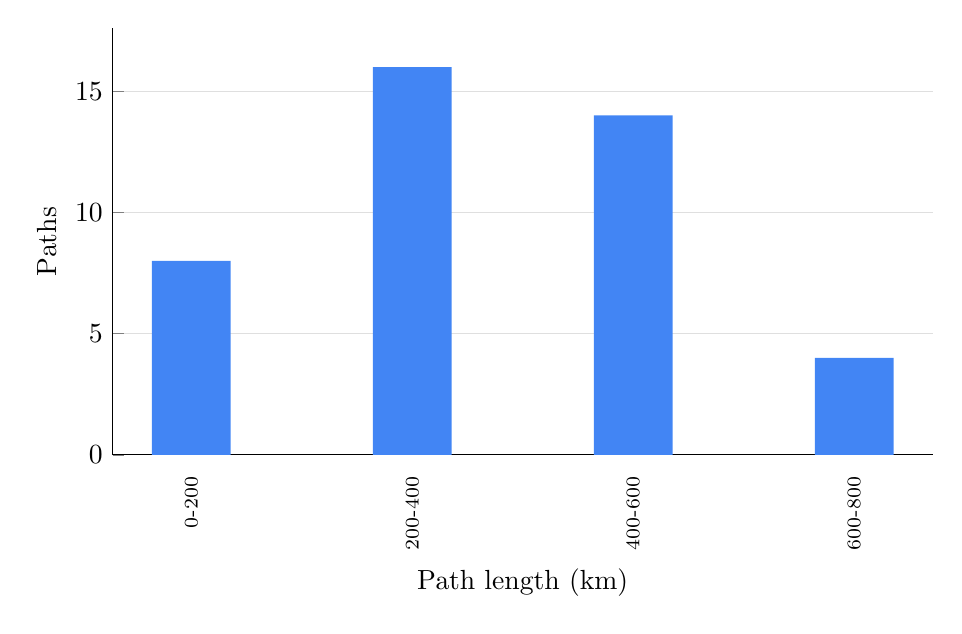
\begin{tikzpicture}
\begin{axis}[
  ybar, bar width=1.000cm, width=12.000cm, height=7cm,
  ymin=0, ymajorgrids, grid style={gray!25}, axis lines*=left,
  enlarge x limits={abs=1.000cm}, xtick=data, major x tick style={draw=none},
  x tick label style={rotate=90, font=\scriptsize, /pgf/number format/1000 sep=},
  legend style={at={(0.5,-0.3)}, anchor=north, legend columns=-1, draw=none},
  ylabel={Paths},
  xlabel={Path length (km)},
  symbolic x coords={0-200,200-400,400-600,600-800,800-1000,1000-1200,1200-1400,1400-1600,1600-1800,1800-2000}]
\addplot[fill={rgb,255:red,66;green,133;blue,244}, draw=none] coordinates {(0-200,8.000) (200-400,16.000) (400-600,14.000) (600-800,4.000) };
\end{axis}
\end{tikzpicture}\end{center}
\clearpage
\section*{Utilization Entropy}
\begin{center}\begin{adjustbox}{max width=\linewidth}
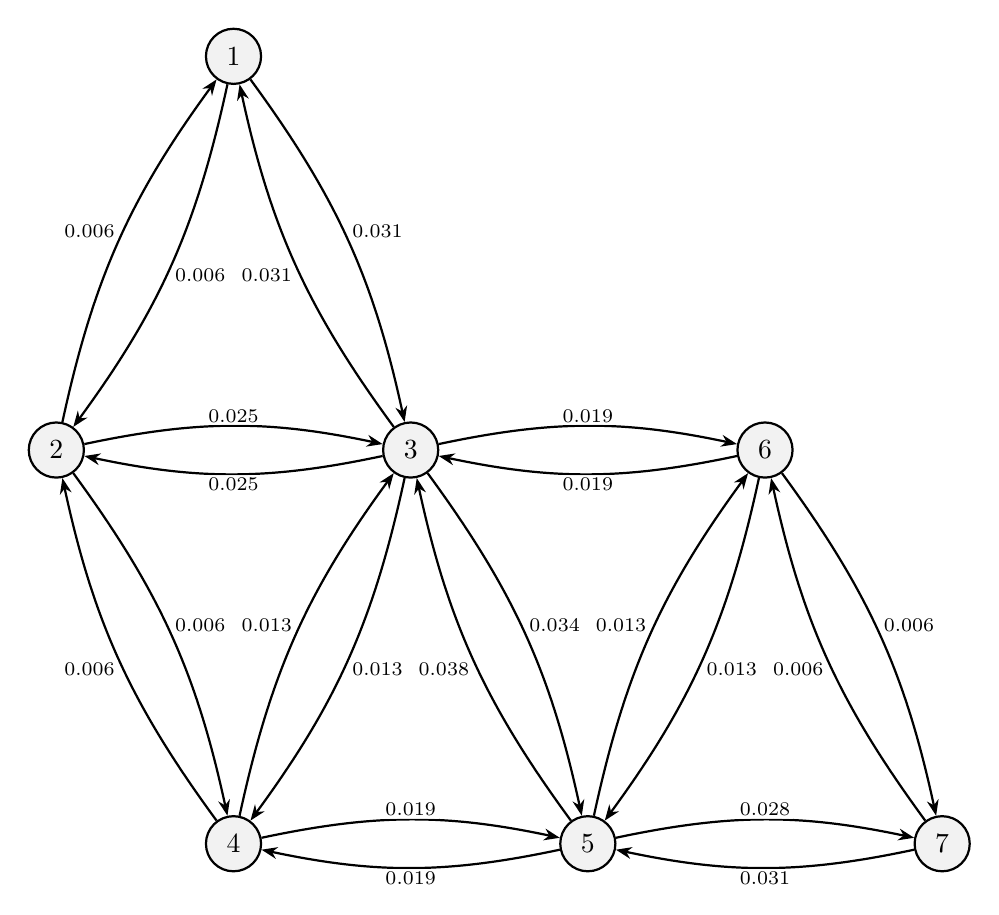
\begin{tikzpicture}[baseline, >={Stealth[length=2mm]},
  netnode/.style={circle, draw, thick, fill=gray!10, minimum size=7mm, inner sep=1pt},
  link/.style={thick},
  linklabel/.style={font=\scriptsize, inner sep=1pt, fill=white, fill opacity=0.85, text opacity=1}]
\node[netnode] (S1) at (2.250,10.000) {1};
\node[netnode] (S2) at (0.000,5.000) {2};
\node[netnode] (S3) at (4.500,5.000) {3};
\node[netnode] (S4) at (2.250,0.000) {4};
\node[netnode] (S5) at (6.750,0.000) {5};
\node[netnode] (S6) at (9.000,5.000) {6};
\node[netnode] (S7) at (11.250,0.000) {7};
\draw[link, ->] (S1) to[bend left=12] node[linklabel, auto] {0.006} (S2);
\draw[link, ->] (S1) to[bend left=12] node[linklabel, auto] {0.031} (S3);
\draw[link, ->] (S2) to[bend left=12] node[linklabel, auto] {0.006} (S1);
\draw[link, ->] (S2) to[bend left=12] node[linklabel, auto] {0.025} (S3);
\draw[link, ->] (S2) to[bend left=12] node[linklabel, auto] {0.006} (S4);
\draw[link, ->] (S3) to[bend left=12] node[linklabel, auto] {0.031} (S1);
\draw[link, ->] (S3) to[bend left=12] node[linklabel, auto] {0.025} (S2);
\draw[link, ->] (S3) to[bend left=12] node[linklabel, auto] {0.013} (S4);
\draw[link, ->] (S3) to[bend left=12] node[linklabel, auto] {0.034} (S5);
\draw[link, ->] (S3) to[bend left=12] node[linklabel, auto] {0.019} (S6);
\draw[link, ->] (S4) to[bend left=12] node[linklabel, auto] {0.006} (S2);
\draw[link, ->] (S4) to[bend left=12] node[linklabel, auto] {0.013} (S3);
\draw[link, ->] (S4) to[bend left=12] node[linklabel, auto] {0.019} (S5);
\draw[link, ->] (S5) to[bend left=12] node[linklabel, auto] {0.038} (S3);
\draw[link, ->] (S5) to[bend left=12] node[linklabel, auto] {0.019} (S4);
\draw[link, ->] (S5) to[bend left=12] node[linklabel, auto] {0.013} (S6);
\draw[link, ->] (S5) to[bend left=12] node[linklabel, auto] {0.028} (S7);
\draw[link, ->] (S6) to[bend left=12] node[linklabel, auto] {0.019} (S3);
\draw[link, ->] (S6) to[bend left=12] node[linklabel, auto] {0.013} (S5);
\draw[link, ->] (S6) to[bend left=12] node[linklabel, auto] {0.006} (S7);
\draw[link, ->] (S7) to[bend left=12] node[linklabel, auto] {0.031} (S5);
\draw[link, ->] (S7) to[bend left=12] node[linklabel, auto] {0.006} (S6);
\end{tikzpicture}
\end{adjustbox}\end{center}

\begin{center}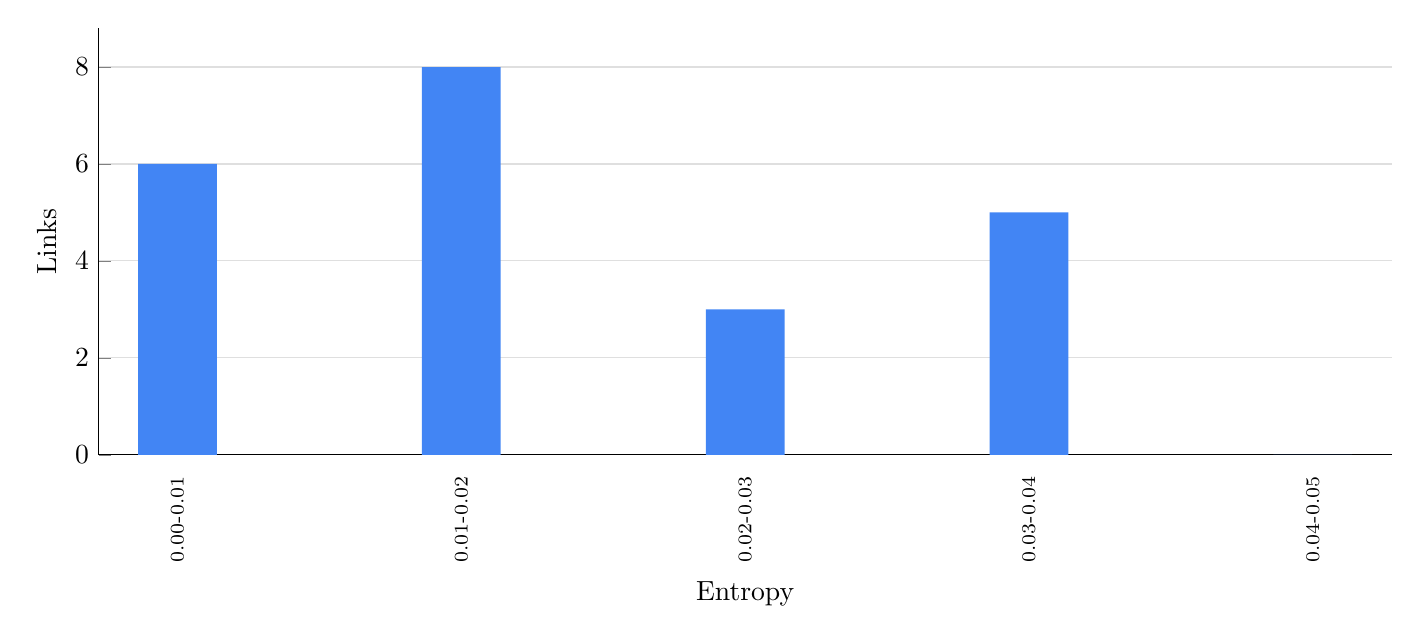
\begin{tikzpicture}
\begin{axis}[
  ybar, bar width=1.000cm, width=18.000cm, height=7cm,
  ymin=0, ymajorgrids, grid style={gray!25}, axis lines*=left,
  enlarge x limits={abs=1.000cm}, xtick=data, major x tick style={draw=none},
  x tick label style={rotate=90, font=\scriptsize, /pgf/number format/1000 sep=},
  legend style={at={(0.5,-0.3)}, anchor=north, legend columns=-1, draw=none},
  ylabel={Links},
  xlabel={Entropy},
  symbolic x coords={0.00-0.01,0.01-0.02,0.02-0.03,0.03-0.04,0.04-0.05,0.05-0.06,0.06-0.07,0.07-0.08,0.08-0.09,0.09-0.10,0.10-0.11,0.11-0.12,0.12-0.13,0.13-0.14,0.14-0.15,0.15-0.16,0.16-0.17,0.17-0.18,0.18-0.19,0.19-0.20,0.20-0.21,0.21-0.22,0.22-0.23,0.23-0.24,0.24-0.25,0.25-0.26,0.26-0.27,0.27-0.28,0.28-0.29,0.29-0.30,0.30-0.31,0.31-0.32,0.32-0.33,0.33-0.34,0.34-0.35,0.35-0.36,0.36-0.37,0.37-0.38,0.38-0.39,0.39-0.40,0.40-0.41,0.41-0.42,0.42-0.43,0.43-0.44,0.44-0.45,0.45-0.46,0.46-0.47,0.47-0.48,0.48-0.49,0.49-0.50,0.50-0.51,0.51-0.52,0.52-0.53,0.53-0.54,0.54-0.55,0.55-0.56,0.56-0.57,0.57-0.58,0.58-0.59,0.59-0.60,0.60-0.61,0.61-0.62,0.62-0.63,0.63-0.64,0.64-0.65,0.65-0.66,0.66-0.67,0.67-0.68,0.68-0.69,0.69-0.70,0.70-0.71,0.71-0.72,0.72-0.73,0.73-0.74,0.74-0.75,0.75-0.76,0.76-0.77,0.77-0.78,0.78-0.79,0.79-0.80,0.80-0.81,0.81-0.82,0.82-0.83,0.83-0.84,0.84-0.85,0.85-0.86,0.86-0.87,0.87-0.88,0.88-0.89,0.89-0.90,0.90-0.91,0.91-0.92,0.92-0.93,0.93-0.94,0.94-0.95,0.95-0.96,0.96-0.97,0.97-0.98,0.98-0.99,0.99-1.00}]
\addplot[fill={rgb,255:red,66;green,133;blue,244}, draw=none] coordinates {(0.00-0.01,6.000) (0.01-0.02,8.000) (0.02-0.03,3.000) (0.03-0.04,5.000) (0.04-0.05,0.000) };
\end{axis}
\end{tikzpicture}\end{center}
\clearpage
\section*{Shannon Entropy}
\begin{center}\begin{adjustbox}{max width=\linewidth}
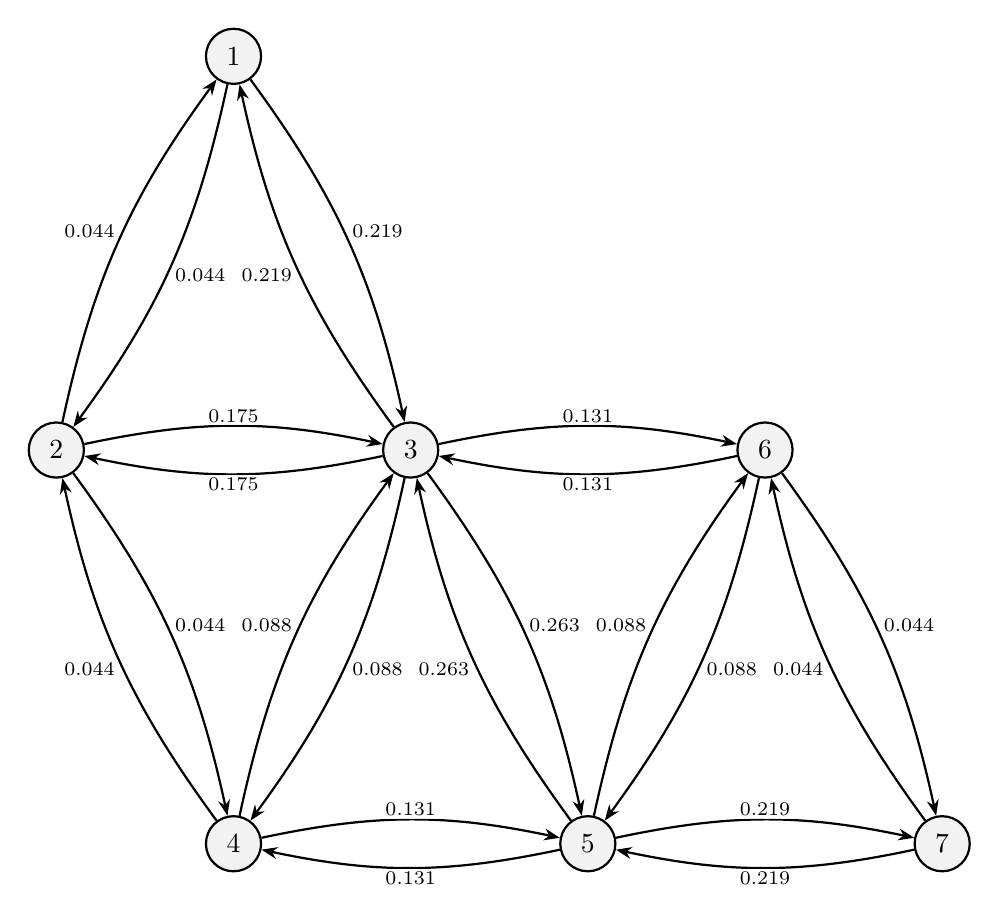
\begin{tikzpicture}[baseline, >={Stealth[length=2mm]},
  netnode/.style={circle, draw, thick, fill=gray!10, minimum size=7mm, inner sep=1pt},
  link/.style={thick},
  linklabel/.style={font=\scriptsize, inner sep=1pt, fill=white, fill opacity=0.85, text opacity=1}]
\node[netnode] (S1) at (2.250,10.000) {1};
\node[netnode] (S2) at (0.000,5.000) {2};
\node[netnode] (S3) at (4.500,5.000) {3};
\node[netnode] (S4) at (2.250,0.000) {4};
\node[netnode] (S5) at (6.750,0.000) {5};
\node[netnode] (S6) at (9.000,5.000) {6};
\node[netnode] (S7) at (11.250,0.000) {7};
\draw[link, ->] (S1) to[bend left=12] node[linklabel, auto] {0.044} (S2);
\draw[link, ->] (S1) to[bend left=12] node[linklabel, auto] {0.219} (S3);
\draw[link, ->] (S2) to[bend left=12] node[linklabel, auto] {0.044} (S1);
\draw[link, ->] (S2) to[bend left=12] node[linklabel, auto] {0.175} (S3);
\draw[link, ->] (S2) to[bend left=12] node[linklabel, auto] {0.044} (S4);
\draw[link, ->] (S3) to[bend left=12] node[linklabel, auto] {0.219} (S1);
\draw[link, ->] (S3) to[bend left=12] node[linklabel, auto] {0.175} (S2);
\draw[link, ->] (S3) to[bend left=12] node[linklabel, auto] {0.088} (S4);
\draw[link, ->] (S3) to[bend left=12] node[linklabel, auto] {0.263} (S5);
\draw[link, ->] (S3) to[bend left=12] node[linklabel, auto] {0.131} (S6);
\draw[link, ->] (S4) to[bend left=12] node[linklabel, auto] {0.044} (S2);
\draw[link, ->] (S4) to[bend left=12] node[linklabel, auto] {0.088} (S3);
\draw[link, ->] (S4) to[bend left=12] node[linklabel, auto] {0.131} (S5);
\draw[link, ->] (S5) to[bend left=12] node[linklabel, auto] {0.263} (S3);
\draw[link, ->] (S5) to[bend left=12] node[linklabel, auto] {0.131} (S4);
\draw[link, ->] (S5) to[bend left=12] node[linklabel, auto] {0.088} (S6);
\draw[link, ->] (S5) to[bend left=12] node[linklabel, auto] {0.219} (S7);
\draw[link, ->] (S6) to[bend left=12] node[linklabel, auto] {0.131} (S3);
\draw[link, ->] (S6) to[bend left=12] node[linklabel, auto] {0.088} (S5);
\draw[link, ->] (S6) to[bend left=12] node[linklabel, auto] {0.044} (S7);
\draw[link, ->] (S7) to[bend left=12] node[linklabel, auto] {0.219} (S5);
\draw[link, ->] (S7) to[bend left=12] node[linklabel, auto] {0.044} (S6);
\end{tikzpicture}
\end{adjustbox}\end{center}

\begin{center}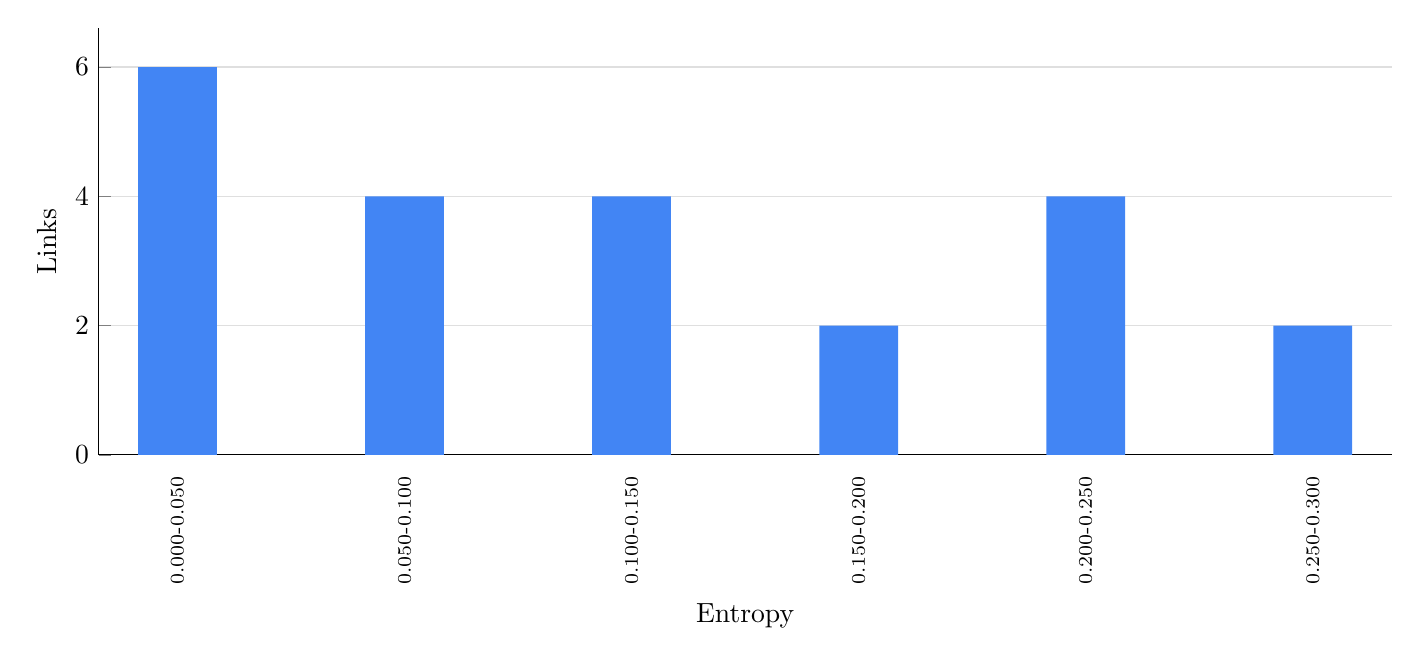
\begin{tikzpicture}
\begin{axis}[
  ybar, bar width=1.000cm, width=18.000cm, height=7cm,
  ymin=0, ymajorgrids, grid style={gray!25}, axis lines*=left,
  enlarge x limits={abs=1.000cm}, xtick=data, major x tick style={draw=none},
  x tick label style={rotate=90, font=\scriptsize, /pgf/number format/1000 sep=},
  legend style={at={(0.5,-0.3)}, anchor=north, legend columns=-1, draw=none},
  ylabel={Links},
  xlabel={Entropy},
  symbolic x coords={0.000-0.050,0.050-0.100,0.100-0.150,0.150-0.200,0.200-0.250,0.250-0.300,0.300-0.350,0.350-0.400,0.400-0.450,0.450-0.500,0.500-0.550,0.550-0.600,0.600-0.650,0.650-0.700,0.700-0.750,0.750-0.800,0.800-0.850,0.850-0.900,0.900-0.950,0.950-1.000}]
\addplot[fill={rgb,255:red,66;green,133;blue,244}, draw=none] coordinates {(0.000-0.050,6.000) (0.050-0.100,4.000) (0.100-0.150,4.000) (0.150-0.200,2.000) (0.200-0.250,4.000) (0.250-0.300,2.000) };
\end{axis}
\end{tikzpicture}\end{center}

\end{document}
